% Created 2020-11-26 四 00:54
% Intended LaTeX compiler: pdflatex
\documentclass[fontset=none,UTF8,a4paper,zihao=-4]{ctexart}
\usepackage[utf8]{inputenc}
\usepackage[T1]{fontenc}
\usepackage{graphicx}
\usepackage{grffile}
\usepackage{longtable}
\usepackage{wrapfig}
\usepackage{rotating}
\usepackage{amsmath}
\usepackage{textcomp}
\usepackage{amssymb}
\usepackage{capt-of}
\usepackage{hyperref}

\setmainfont{Times New Roman}
\setCJKmainfont[ItalicFont={楷体}]{宋体}
\setCJKsansfont{微软雅黑}
\setCJKmonofont{微软雅黑}


%%% 默认使用的latex宏包 %%%
\usepackage{tikz}
\usepackage{CJKulem}
\usepackage{graphicx}

%%% 设置页面边距 %%%
\usepackage[top=2.54cm, bottom=2.54cm, left=3.17cm, right=3.17cm]{geometry} %
\author{LGT}
\date{\textit{<2020-11-25 三>}}
\title{SLR文法分析程序Readme}
\hypersetup{
 pdfauthor={LGT},
 pdftitle={SLR文法分析程序Readme},
 pdfkeywords={},
 pdfsubject={},
 pdfcreator={Emacs 28.0.50 (Org mode 9.5)}, 
 pdflang={English}}
\begin{document}

\maketitle
\tableofcontents


\section{运行截图}
\label{sec:org2d65b66}
\begin{itemize}
\item 文法串识别和 FIRST/FOLLOW

\begin{center}
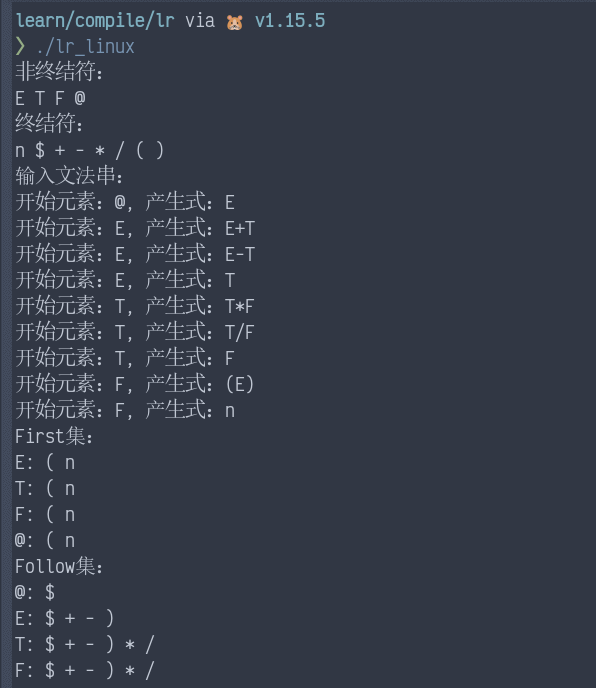
\includegraphics[width=.9\linewidth]{运行截图/2020-11-26_00-44-40_screenshot.png}
\end{center}

\item 求得的项目族

\begin{center}
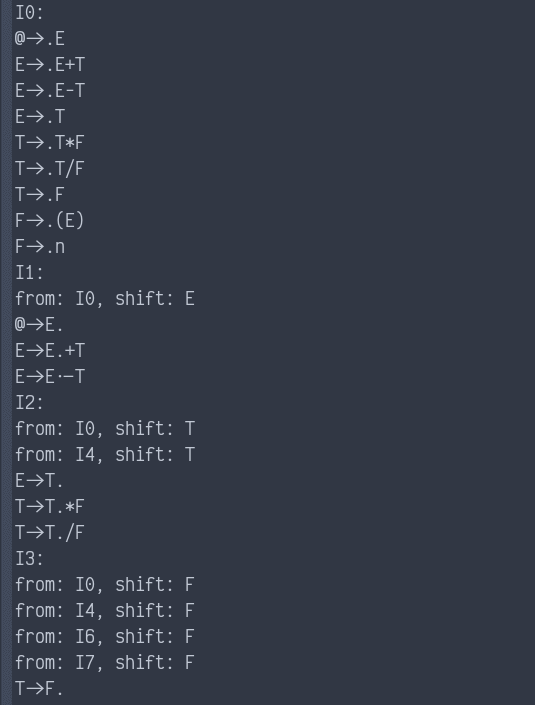
\includegraphics[width=.9\linewidth]{运行截图/2020-11-26_00-45-19_screenshot.png}
\end{center}

\begin{center}
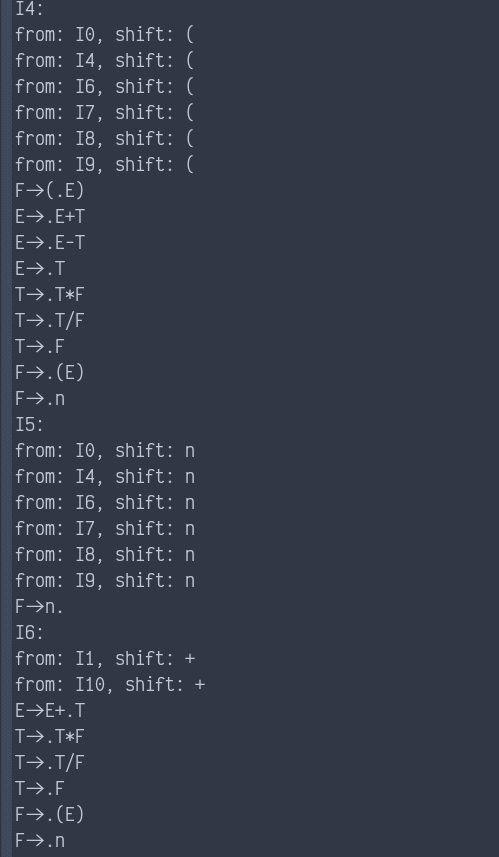
\includegraphics[width=.9\linewidth]{运行截图/2020-11-26_00-45-36_screenshot.png}
\end{center}

\begin{center}
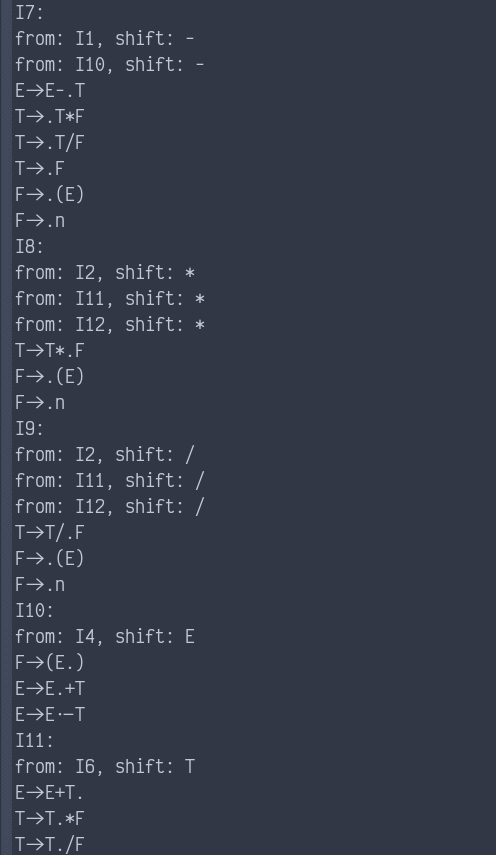
\includegraphics[width=.9\linewidth]{运行截图/2020-11-26_00-46-53_screenshot.png}
\end{center}

\begin{center}
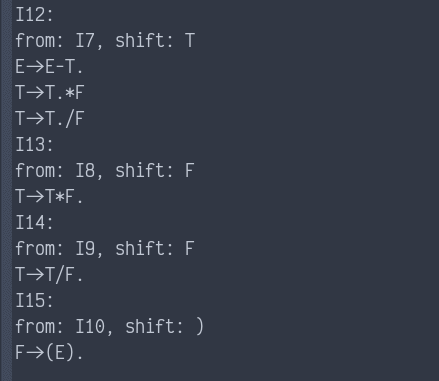
\includegraphics[width=.9\linewidth]{运行截图/2020-11-26_00-47-20_screenshot.png}
\end{center}

\item 文法分析表

\begin{center}
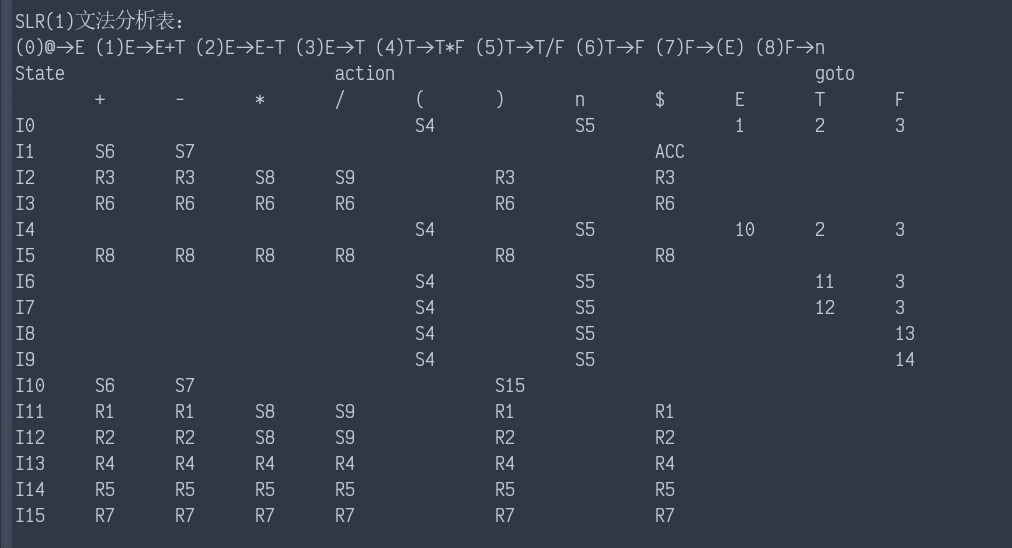
\includegraphics[width=.9\linewidth]{运行截图/2020-11-26_00-54-22_screenshot.png}
\end{center}
\end{itemize}


\begin{itemize}
\item 待约串分析动作表

\begin{center}
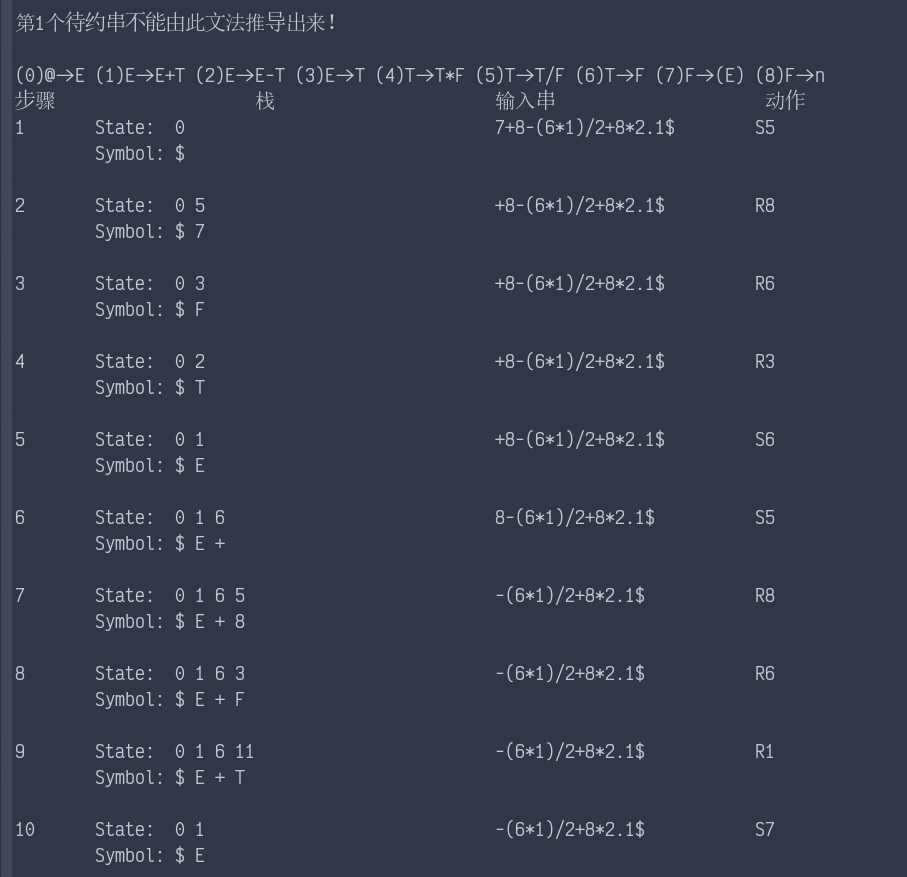
\includegraphics[width=.9\linewidth]{运行截图/2020-11-26_00-48-40_screenshot.png}
\end{center}

\begin{center}
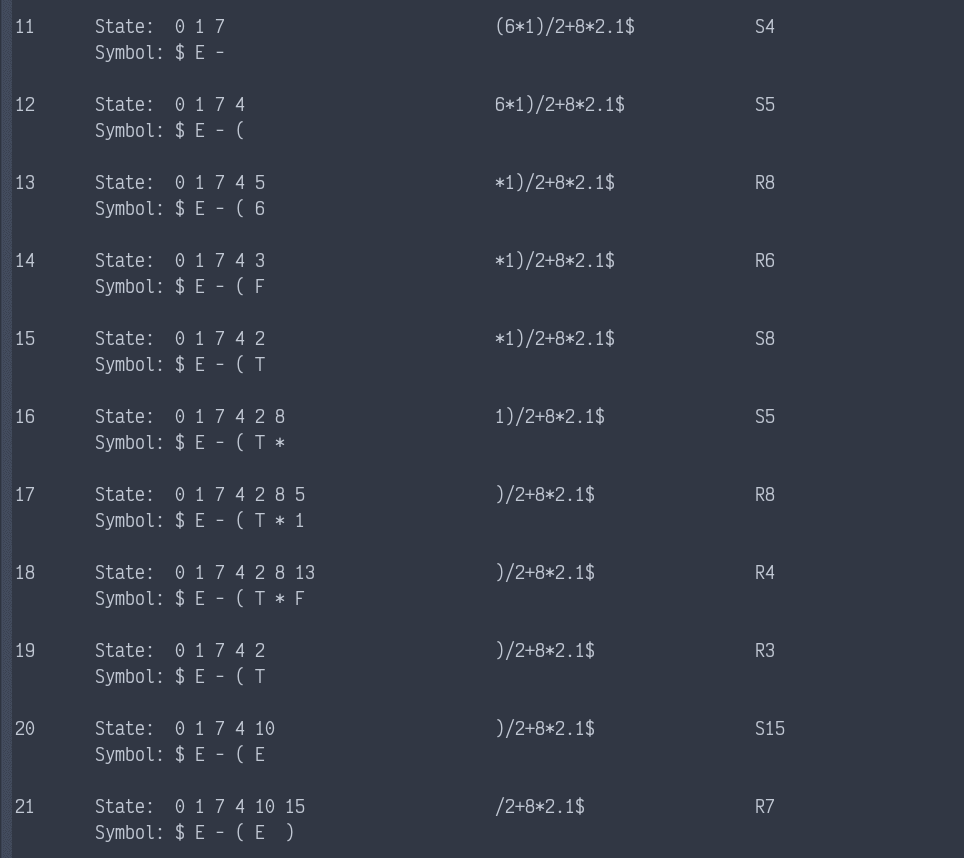
\includegraphics[width=.9\linewidth]{运行截图/2020-11-26_00-49-00_screenshot.png}
\end{center}

\begin{center}
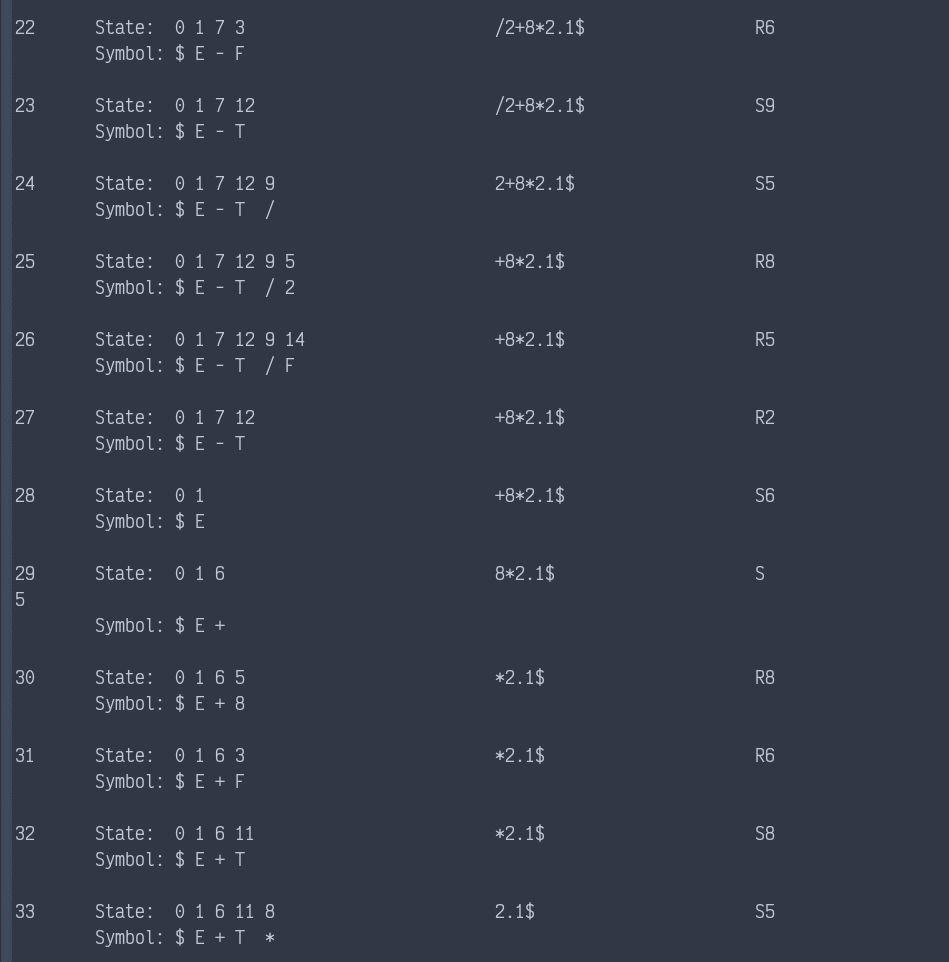
\includegraphics[width=.9\linewidth]{运行截图/2020-11-26_00-49-14_screenshot.png}
\end{center}

\begin{center}
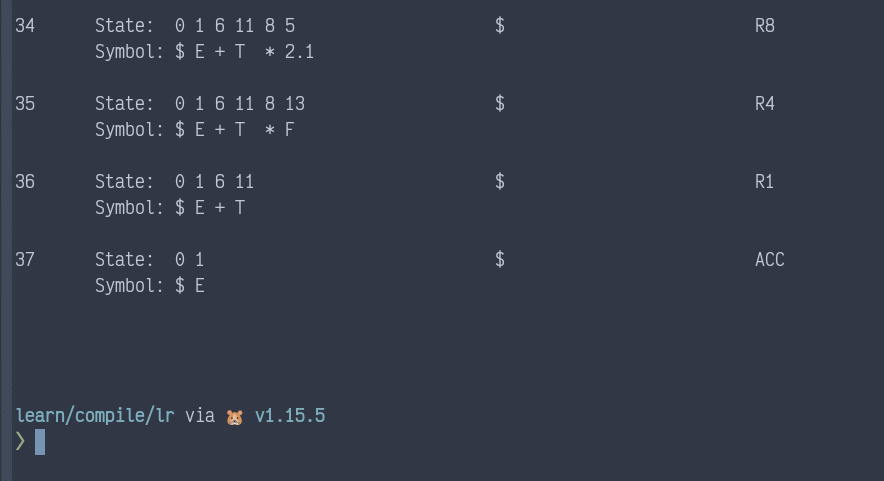
\includegraphics[width=.9\linewidth]{运行截图/2020-11-26_00-49-23_screenshot.png}
\end{center}
\end{itemize}

\section{如何运行}
\label{sec:org99a2ae6}
\begin{itemize}
\item Windows

点击 lr.exe 即可

\item Linux

./lr\_linux

\item MacOS

./lr\_mac
\end{itemize}


\section{程序功能}
\label{sec:org53df831}
\begin{enumerate}
\item 读取存储满足要求的文法串的文件

文法的要求:
\begin{enumerate}
\item 设计正确的 SLR(1)文法
\item 文法串中的大写字母表示非终结符,小写字母(除 n)和符号(除@)表示终结符,n表示数字
\item 不同文法串用换行符分隔
\end{enumerate}
\item 分析输入的文法串
\begin{enumerate}
\item 输出文法中的非终结符和终结符
\item 输出文法中非终结符的 FIRST, FOLLOW 集
\item 输出 SLR(1)形式的文法项目族
\item 输出 SLR(1)形式的分析表
\end{enumerate}
\item 读取存储待约串的文件(不同待约串按行分隔)
\item 输出所有待约串的分析过程(可以检测无法推出的待约串)
\end{enumerate}

\section{程序逻辑}
\label{sec:org38ebe3d}
\begin{enumerate}
\item 读取输入的文法串
\item 求输入文法串的 FIRST/FOLLOW 集
\item 求文法规范项目族
\item 求文法分析表
\item 读取输入的待约串集
\item 对每一条待约串进行语法分析并输出分析动作表
\end{enumerate}

\section{程序结构体}
\label{sec:org5342c77}
\begin{enumerate}
\item expMap: 存储文法串
\begin{itemize}
\item start:  文法串的开始符号
\item subExp: 文法串的产生式
\end{itemize}
\item source: 用来确定来源项目集
\begin{itemize}
\item from:  项目集来源的序号
\item shift: 移进的符号
\end{itemize}
\item solu: 项目集
\begin{itemize}
\item sources: 此项目集的来源
\item list:    此项目集中的文法串
\item isTran:  项目集中的文法串是否被遍历
\end{itemize}
\item place: 二维序号
\begin{itemize}
\item x: 项目集序号
\item y: 项目集中产生式序号
\end{itemize}
\item table: 文法分析表
\begin{itemize}
\item action: action 表
\item goTo: goto 表
\end{itemize}
\item stack: 状态符号栈
\begin{itemize}
\item state:  状态
\item symbol: 符号
\end{itemize}
\item doline: 分析动作表的一行
\begin{itemize}
\item no: 步骤
\item st: 状态符号栈
\item s:  当前状态下的剩余符号串
\item do: 分析动作
\end{itemize}
\end{enumerate}

\section{程序全局变量}
\label{sec:org2485ddc}
\begin{enumerate}
\item oriBegin:    拓广之前的文法开始符号
\item begin:       拓广之后的文法开始符号
\item beginSubExp: 拓广之后的文法开始符号的产生式
\item vCnt:        非终结符计数
\item tCnt:        终结符计数
\item vs:          非终结符的 map
\item ts:          终结符的 map
\item exps:        文法串数组
\item first:       文法 FIRST 集
\item follow:     文法 FOLLOW 集
\item flag:       标志某非终结符(用于求 FOLLOW 集)
\item solus:      文法项目族
\item aTable:     文法分析表
\item inputArr:   输入待约串集
\item cInput:     当前规约串
\item aDoTable:   分析动作表
\end{enumerate}


\section{程序函数}
\label{sec:orgc9dc469}
\begin{enumerate}
\item push(st stack, sta int, sym string) stack

\begin{itemize}
\item 用途

将新的状态和栈顶符号压栈

\item 参数

st: 要操作的栈

sta: 新的栈顶状态

sym: 新的栈顶符号

\item 返回值

压栈之后的栈
\end{itemize}

\item pop(st stack) stack

\begin{itemize}
\item 用途

弹栈

\item 参数

st: 要进行弹栈操作的栈

\item 返回值

弹栈之后的栈
\end{itemize}

\item peek(st stack) (int, string)

\begin{itemize}
\item 用途

返回栈顶状态和符号

\item 参数

要求栈顶状态和符号的栈

\item 返回值

int:    栈顶状态
string: 栈顶符号
\end{itemize}

\item isEmpty(st stack) bool

\begin{itemize}
\item 用途

判断栈是否为空

\item 参数

要判断的栈

\item 返回值

栈是否为空
\end{itemize}

\item subPeekSta(st stack, popLen int) int

\begin{itemize}
\item 用途

返回规约之后的次栈顶状态

\item 参数

st:     要分析的栈

popLen: 规约产生式的长度

\item 返回值

规约之后的次栈顶状态
\end{itemize}

\item analysis()

\begin{itemize}
\item 用途

分析待约串集合
\end{itemize}

\item getDoTable(input string) (error, int)

\begin{itemize}
\item 用途

得到当前待约串的分析动作表

\item 参数

input: 当前待约串

\item 返回值

error: 分析过程中发生的错误

int:   发生错误的位置
\end{itemize}

\item distNum(offset int, term string, isNum bool) (error, int)

\begin{itemize}
\item 用途

区别当前符号是否数字的同时,构造一条分析动作

\item 参数

offset: 当前符号的长度

term: 当前符号

isNum: 是否为数字

\item 返回值

error: 分析过程中发生的错误

int:   发生错误的位置
\end{itemize}

\item getADoline(input string, no int) doline

\begin{itemize}
\item 用途

构造一个基础的分析动作

\item 参数

input: 此动作对应的剩余分析串

no:    此动作对应的步骤

\item 返回值

doline: 构造好的分析动作
\end{itemize}

\item cut(s string) (int, res string, kind string)

\begin{itemize}
\item 用途

截取当前剩余的符号串

\item 参数

s: 当前的剩余符号串

\item 返回值

int:  截取出的符号的长度

res:  截取出的符号

kind: 截取出符号的类型
\end{itemize}

\item readInput(fName string)

\begin{itemize}
\item 用途

从文件读取待约符号串集

\item 参数

存储待约符号串集的文件名
\end{itemize}

\item initialize()

\begin{itemize}
\item 用途

初始化需要初始化的全局变量
\end{itemize}

\item readGrammar(fName string)

\begin{itemize}
\item 用途

从文件读取文法集

\item 参数

存储文法集的文件名
\end{itemize}

\item outputGrammar()

\begin{itemize}
\item 用途

输出文法相关信息
\end{itemize}

\item getTable()

\begin{itemize}
\item 用途

生成文法分析表
\end{itemize}

\item mapSubExp(subExp string) int

\begin{itemize}
\item 用途

映射产生式和序号

\item 参数

产生式

\item 返回值

产生式的序号
\end{itemize}

\item mapShift(shift rune, isT bool) int

\begin{itemize}
\item 用途

映射终结符/非终结符的序号

\item 参数

shift: 符号

isT:  是否为终结符

\item 返回值

符号对应的序号
\end{itemize}

\item findTo(from int, shift rune) int

\begin{itemize}
\item 用途

获取要到达的项目集序号

\item 参数

from:  起始项目集的序号
shift: 当前移进的符号

\item 返回值

int: 要到达的项目集的符号
\end{itemize}

\item getClosure()

\begin{itemize}
\item 用途

获取文法的项目族
\end{itemize}

\item isSoluExist(list []expMap) (bool, int)

\begin{itemize}
\item 用途

判断此项目集是否已经在项目族中存在

\item 参数

list: 要进行判断的项目集

\item 返回值

bool: 是否存在
int:  如果存在即为与之相同的项目集编号
\end{itemize}

\item isEnd(isBack bool) (bool, place)

\begin{itemize}
\item 用途

判断是否遍历完整个项目族

\item 参数

isBack: 是否用来求文法分析表

\item 返回值

bool:  遍历是否结束
place: 当前未被遍历的项目集中产生式的位置
\end{itemize}

\item closure(iMap expMap) []expMap

\begin{itemize}
\item 用途

求某个产生式对应的闭包

\item 参数

iMap: 产生式

\item 返回值

[]expMap: 此产生式对应的闭包
\end{itemize}

\item getNextMap(start rune) []expMap

\begin{itemize}
\item 用途

获得下一个要求闭包的产生式集

\item 参数

start: 产生式的开始符号

\item 返回值

[]expMap: 开始符号对应的产生式集
\end{itemize}

\item addDot(p int, oriExp string) string

\begin{itemize}
\item 用途

为没有加点的产生式加点

\item 参数

p:      加点的位置
oriExp: 要加点的产生式

\item 返回值

string: 加点之后的产生式
\end{itemize}

\item moveDot(p int, oriExp string) string

\begin{itemize}
\item 用途

将有点的产生式中的点向后移动一位

\item 参数

p: 点在产生式中的位置

oriExp: 要移动点位置的产生式

\item 返回值

string: 移动点之后的产生式
\end{itemize}

\item firstAndFollow()

\begin{itemize}
\item 用途

构造并输出 FIRST, FOLLOW 集
\end{itemize}

\item getFirst(start rune) []rune

\begin{itemize}
\item 用途

求 FIRST 集

\item 参数

start: 要求 FIRST 集的非终结符

\item 返回值

[]rune: start 对应的 FIRST 集
\end{itemize}

\item getFollow(start rune) []rune

\begin{itemize}
\item 用途

求 FOLLOW 集

\item 参数

start: 要求 FOLLOW 集的非终结符

\item 返回值

[]rune: start 对应的 FOLLOW 集
\end{itemize}

\item isExist(c rune, cArr map[int]rune) bool

\begin{itemize}
\item 用途

判断符号是否存在

\item 参数

c:    要进行判断的符号
cArr: 符号对应的 map

\item 返回值

bool: 符号是否存在
\end{itemize}

\item getVT(iStr string)

\begin{itemize}
\item 用途

求非终结符和非终结符

\item 参数

iStr: 要进行分析的文法串
\end{itemize}

\item printChar(charMap map[int]rune)

\begin{itemize}
\item 用途

打印识别出的符号

\item 参数

符号对应的 map
\end{itemize}

\item printStr(strArr []string)

\begin{itemize}
\item 用途

打印字符串集合

\item 参数

strArr: 字符串集合
\end{itemize}

\item printExpMap(expArr []expMap)

\begin{itemize}
\item 用途

打印文法

\item 参数

expArr: 文法集合
\end{itemize}

\item printF(f map[rune][]rune)

\begin{itemize}
\item 用途

打印 FIRST, FOLLOW 集

\item 参数

FIRST/FOLLOW 集
\end{itemize}

\item printClosure()

\begin{itemize}
\item 用途

打印闭包
\end{itemize}

\item printTable()

\begin{itemize}
\item 用途

打印文法分析表
\end{itemize}

\item getMaxStLen() int

\begin{itemize}
\item 用途

获取当前动作分析表中最大栈长度

\item 返回值

当前动作分析表中最大栈长度
\end{itemize}

\item printDoTable()

\begin{itemize}
\item 用途

打印动作分析表
\end{itemize}
\end{enumerate}
\end{document}
